\section{Nota teórica}
En esta sección se describen los componentes principales que se utilizaron para el desarrollo del HAR-Human Activity Recognition.
\subsection*{ Arduino Nano 33 BLE}
El arduino Nano 33 BLE Sense es un módulo miniatura que contiene un módulo NINA B306, basado en Nordic nRF52480 y contiene un M4F Cortex, un cripto chip el cual puede almacenar certficados de forma segura y pre-compartir llaves y un IMU de 9 ejes. El módulo puede ser montado como un componente DIP o como componente SMT, directamente soldado por la via de los pads.
\subsubsection*{Características generales}
Las características más importantes de este mcu se mencionan a continuación \cite{web}
\begin{multicols}{2}
 \begin{itemize}
    \item CPU: ARM Cortex-M4 a 64MHz con FPU, 32-bit, 1MB Flash, 256kB SRAM.
    \item Bluetooth 5, IEEE 802.15.4-2006, \SI{2.4}{\giga\Hz}.
    \item ARM TrusZone Cryptocell 310 security subsystem, secure boot.
    \item USB 2.0, QSPI, SPI.
    \item 48 GPIOs.
    \item 12-bit, ADC con 8 canales.
    \item 64 comparadores de nivel, 15 del tipo low-power.
    \item Sensor de temperatura.
    \item $4\times4$-canales PWM.
    \item Periféricos de audio: I2S, PDM
    \item $5\times32$-bit timers.
    \item $4\times$ SPI maestros\/$3\times$ SPI esclavos.
    \item $2\times$I2C.
    \item $2\times$ UART.
    \item decodificador de cuadratura (QDEC).
    \item $3\times$ RTC.
\end{itemize}   
\end{multicols}
\newpage
\subsubsection*{Diagrama de bloques}
La figura \ref{fig1} representa el diagrama de bloques de la placa.
\begin{figure}[H]
\centering
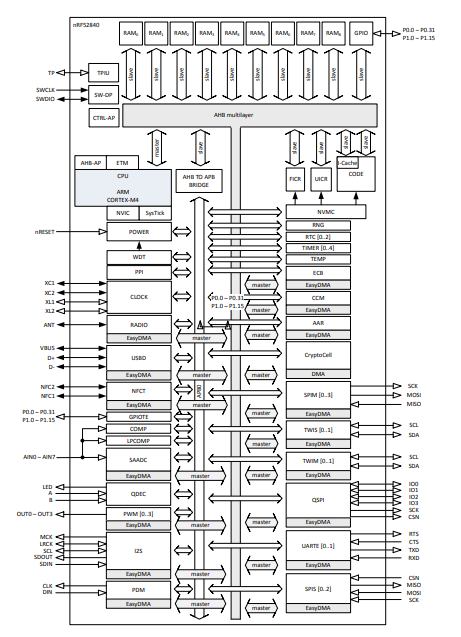
\includegraphics[width=.55\linewidth]{Imagenes/1.png}
 \caption{Diagrama de bloques del Nano BLE 33 Sense . Tomado de \cite{web}.}
 \label{fig1}
\end{figure}
\newpage
\subsubsection*{Diagrama de pines}
El diagrama de la fugura \ref{fig2} brinda de manera más detallada la distribución de los pines.
\begin{figure}[H]
\centering
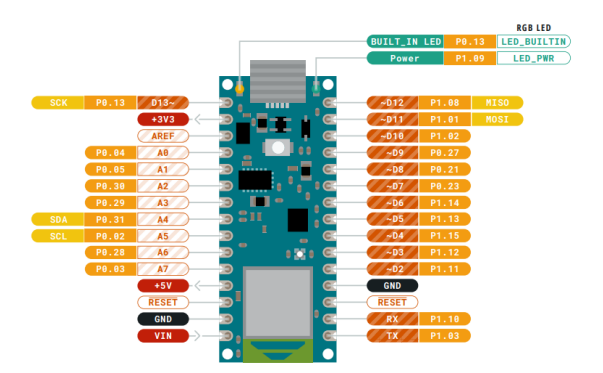
\includegraphics[width=.55\linewidth]{Imagenes/2.png}
 \caption{Diagrama de pines del Nano BLE 33 Sense . Tomado de \cite{web2}.}
 \label{fig2}
\end{figure}
\subsubsection*{Características eléctricas}
Aquí se tomaron dos referencias para tener más claro este detalle,  primero se muestran los valores máximos del mcu nRF52480 y los de la placa respectivamente.
\begin{figure}[H]
\centering
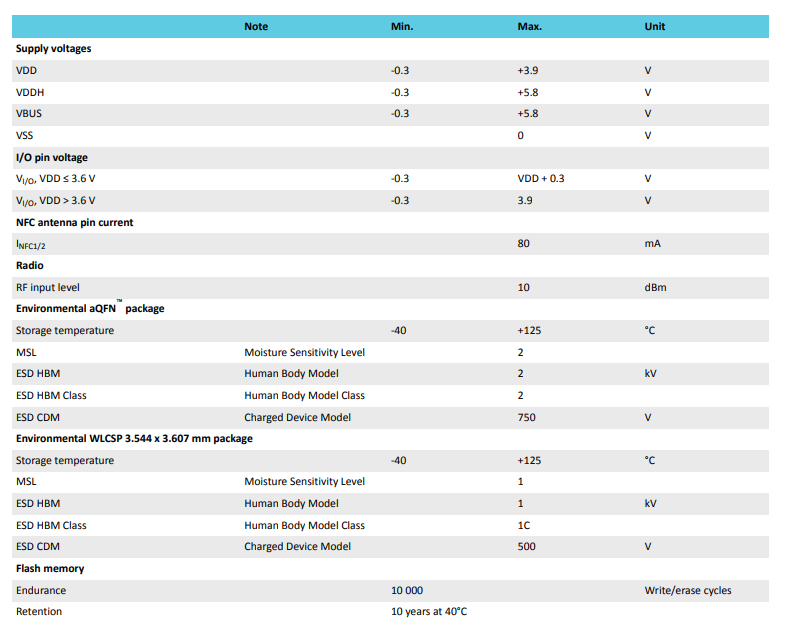
\includegraphics[width=.55\linewidth]{Imagenes/3.png}
 \caption{Características eléctricas de nRF52480. Tomado de \cite{web}.}
 \label{fig3}
 
\end{figure}
\begin{figure}[H]
\centering
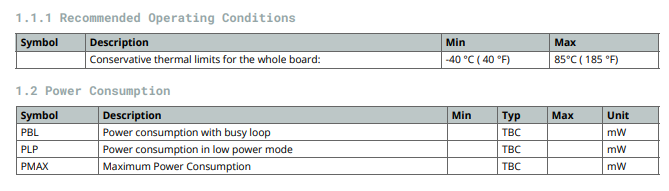
\includegraphics[width=.55\linewidth]{Imagenes/3.1.png}
 \caption{ Características eléctricas de la placa. Tomado de \cite{web2}.}
 \label{fig3.1}
\end{figure}


\subsection*{Periféricos utilizados}
En este laboratorio no se utilizaron periféricos externos, además, el único sensor que se utilizó es el giroscopio de 9 ejes que viene incorporado en el Arduino Nano 33 BLE. A continuación se presentan los puntos más importantes de este sensor (LSM9DS1) para realizar este laboratorio \cite{giroscopio}:
\begin{itemize}
    \item 3 canales de aceleración, 3 canales de velocidad angular, 3 canales de campo magnético.
    \item ±2/±4/±8/±16 g aceleración lineal escala completa.
    \item ±245/±500/±2000 dps velocidad angular escala completa.
    \item Salida de datos de 16 bits.
    \item Interfaces serie SPI / I2C.
    \item Tensión de alimentación analógica 1,9 V a 3,6 V.
\end{itemize}

\begin{figure}[H]
    \centering
    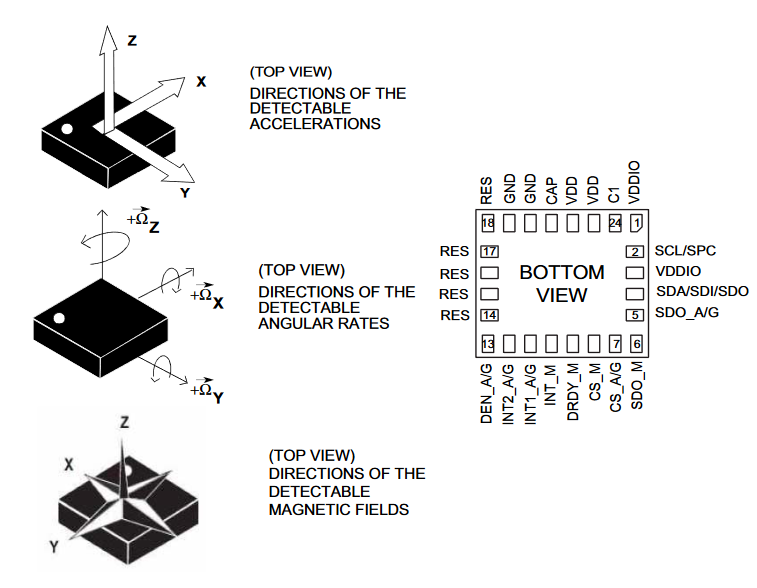
\includegraphics[width=.55\linewidth]{Imagenes/k1.png}
    \caption{Diagrama de pines del LSM9DS1, tomado de \cite{giroscopio}.}
    \label{k1}
\end{figure}


\subsection*{Lista de componentes}
\begin{table}[H]
\caption{Lista de equipos}
\label{table_2}
\begin{center}
\begin{tabular}{r|cc}
\hline
\textbf{Componente}&\textbf{Cantidad}&\textbf{Precio}\\
 \hline
Arduino Nano 33 BLE & 1 & 60\$ \\ \hline 

 \textbf{Total}& & 60\$ \\
 \hline
\end{tabular}
\end{center}
\end{table}

\subsection*{Diseño del circuito}
El diseño del circuito es muy simple ya que basta con conectar el arduino nano 33 ble sense a la computadora por medio de un cable USB, tal como se muestra en la figura \ref{fig4}.
\begin{figure}[H]
\centering


\tikzset{every picture/.style={line width=0.75pt}} %set default line width to 0.75pt        

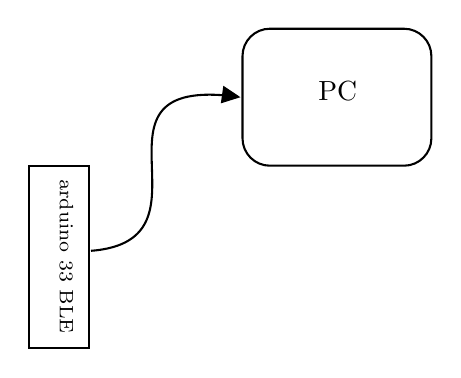
\begin{tikzpicture}[x=0.75pt,y=0.75pt,yscale=-1,xscale=1]
%uncomment if require: \path (0,528); %set diagram left start at 0, and has height of 528

%Shape: Rectangle [id:dp7327399467778912] 
\draw   (233,206) -- (233,294) -- (204,294) -- (204,206) -- cycle ;
%Rounded Rect [id:dp2315563507614331] 
\draw   (307,153.2) .. controls (307,145.91) and (312.91,140) .. (320.2,140) -- (384.8,140) .. controls (392.09,140) and (398,145.91) .. (398,153.2) -- (398,192.8) .. controls (398,200.09) and (392.09,206) .. (384.8,206) -- (320.2,206) .. controls (312.91,206) and (307,200.09) .. (307,192.8) -- cycle ;
%Curve Lines [id:da34814740280768275] 
\draw    (234,247) .. controls (298.35,242.05) and (224.51,162.61) .. (303.56,172.67) ;
\draw [shift={(306,173)}, rotate = 188.23] [fill={rgb, 255:red, 0; green, 0; blue, 0 }  ][line width=0.08]  [draw opacity=0] (8.93,-4.29) -- (0,0) -- (8.93,4.29) -- cycle    ;

% Text Node
\draw (342,164) node [anchor=north west][inner sep=0.75pt]   [align=left] {PC};
% Text Node
\draw (227,211) node [anchor=north west][inner sep=0.75pt]  [rotate=-90] [align=left] {{\scriptsize arduino 33 BLE}};
\end{tikzpicture}
\caption{ Diagrama del circuito.}
\label{fig4}
\end{figure}
A partir de lo mostrado anteriormente se consultaron las referencias dadas por el profesor para realizar el laboratorio.
\newpage